\documentclass[a4paper]{article}

\usepackage{amsmath}
\usepackage{hyperref}

\usepackage{graphicx}
\usepackage{listings}
\usepackage{color}
 
\definecolor{codegreen}{rgb}{0,0.6,0}
\definecolor{codegray}{rgb}{0.5,0.5,0.5}
\definecolor{codepurple}{rgb}{0.58,0,0.82}
\definecolor{backcolour}{rgb}{0.95,0.95,0.92}
 
\lstdefinestyle{mystyle}{
    backgroundcolor=\color{backcolour},   
    commentstyle=\color{codegreen},
    keywordstyle=\color{magenta},
    numberstyle=\tiny\color{codegray},
    stringstyle=\color{codepurple},
    basicstyle=\footnotesize,
    breakatwhitespace=false,         
    breaklines=true,                 
    captionpos=b,                    
    keepspaces=true,                 
    numbers=left,                    
    numbersep=5pt,                  
    showspaces=false,                
    showstringspaces=false,
    showtabs=false,                  
    tabsize=2
}
 
\lstset{style=mystyle}


\title{Assignment 2: Linear Predictive Analysis}
\author{Pranav Sankhe| 150070009}
\date{4/10/2018}

\begin{document}

\maketitle

\section{Question}
Synthesized vowel: Consider the synthesized vowel /a/ (formants: 730, 1090, 2440 Hz; bandwidths: 50 Hz) at two fundamental frequencies: 120 Hz, 300 Hz. Sampling rate = 8 kHz. Using a 30 ms Hamming window, implement LP analysis on a single segment using LP orders 2, 4, 6, 8, 10 using the Levinson algorithm. Compute the gain, and plot the LP spectrum magnitude (i.e. the dB magnitude frequency response of the estimated all-pole filter) for each order "p". Superimpose each plot on the original 6-pole spectral envelope with the discrete harmonic components shown with vertical lines. Comment on the characteristics of the spectral approximations of different orders.

\subsection{Answer}

\begin{figure}[h!]
    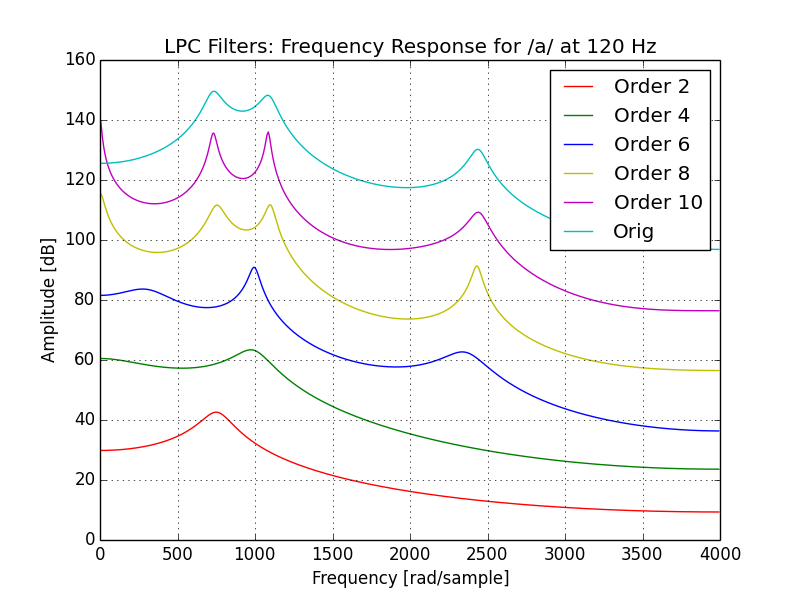
\includegraphics[width=\linewidth]{./images/120.png}
    \caption{ \textbackslash a\textbackslash at $120$ Hz}
    \label{fig:1}
\end{figure}


\begin{figure}[h!]
    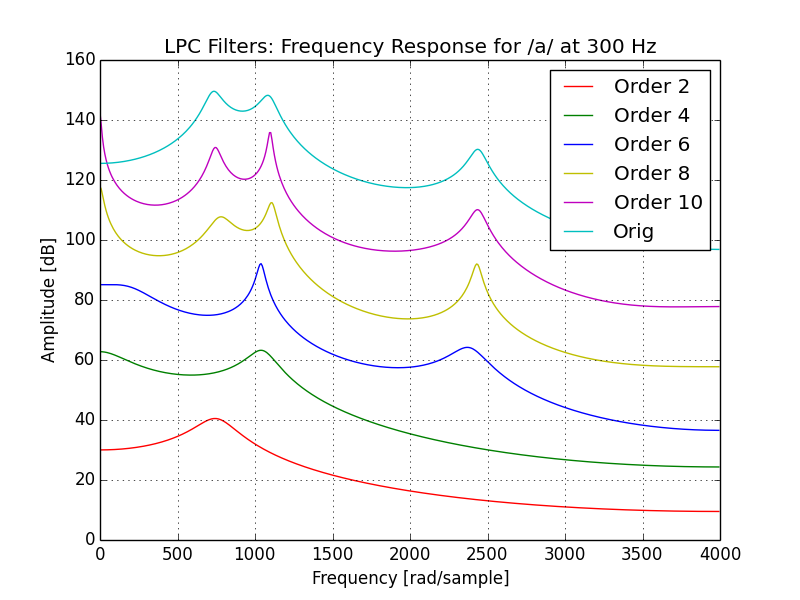
\includegraphics[width=\linewidth]{./images/300.png}
    \caption{ \textbackslash a\textbackslash at $300$ Hz}
    \label{fig:1}
\end{figure}


It is evident from the graphs that the approximation of the real spectrum keeps on getting better as we increase the order at both the signal frequencies. This is expected since as we increase the order, the LP spectrum is able to capture more and more details of the original spectrum. 
Also, as we increase the number of poles (order) we observe that there's an increase in the sharpness of the peaks. \\ 

File containing all the paramaters:
\begin{lstlisting}[language=Python, caption=hparams.py]
formant_freq = [730, 1090, 2440]
formant_bw = [100, 100, 100]
samp_freq = 8000.0
sig_freq = 300
time_length = 0.5
win_size = 30.0
dft_len = 1024
filter_order= [2, 4, 6, 8, 10]
\end{lstlisting}

main file: 

\begin{lstlisting}[language=Python, caption=q1.py]
import librosa
import numpy as np 
from matplotlib import pyplot as plt
import pylab
from scipy import signal
from scipy.io.wavfile import write
import hparams
import sys
from math import pi


def autocorr(x):
    result = np.correlate(x, x, mode='full')
    return result[int(result.size/2):]


sig_freq = hparams.sig_freq

y, samp_freq = librosa.load( str(sig_freq) + '.wav',sr=None)
win_size = hparams.win_size/1000.0 
num_samples = int(samp_freq*win_size)
window = y[:num_samples]*np.hamming(num_samples)

fig1 = plt.figure()
plt.title('LPC Filters: Frequency Response for /a/ at '+str(sig_freq)+' Hz')
plt.ylabel('Amplitude [dB]')
plt.xlabel('Frequency [rad/sample]')

colors = {2: 'r', 4: 'g', 6: 'b', 8: 'y', 10: 'm'}
orders = hparams.filter_order

for order in orders:
    
    R = autocorr(window)
    error = np.zeros(order+1)
    error[0] = R[0]
    G = np.zeros(order + 1)

    coeffs = np.zeros(order+1)
    dummy_coeffs = np.zeros(order + 1)
    

    for i in range(1, order +1):
        reflec_coeffs = 0
        dummy_coeffs[1:len(coeffs)] = coeffs[1:len(coeffs)]
        
        for j in range(1, i):
            reflec_coeffs = reflec_coeffs + dummy_coeffs[j]*R[i-j]
        reflec_coeffs = (R[i] - reflec_coeffs)/error[i-1]

        coeffs[i] = reflec_coeffs

        for j in range(1, i):
            coeffs[j] = dummy_coeffs[j] - reflec_coeffs*dummy_coeffs[i-j]

        error[i] = (1-np.square(reflec_coeffs))*error[i-1]

    coeffs[0] = 1.0
    coeffs[1:len(coeffs)] = -coeffs[1:len(coeffs)]
    num_coeffs = np.zeros(coeffs.shape)
    num_coeffs[0] = 1
    G[i] = np.sqrt(error[i])
    w, h = signal.freqz(num_coeffs, coeffs)

    plt.plot(samp_freq*w/(2*np.pi), 10*order + 20 * np.log10(abs(h)), colors[order])

formant_freq = hparams.formant_freq
formant_bw = hparams.formant_bw

r = np.exp(np.multiply(-np.pi, formant_bw)/samp_freq)
theta = 2*np.multiply(np.pi, formant_freq)/samp_freq

poles = np.concatenate([r * np.exp(1j*theta), r * np.exp(-1j*theta)])
zeros = np.zeros(poles.shape, poles.dtype)

b, a = signal.zpk2tf(zeros, poles, 1)

wf, hf = signal.freqz(b, a)

plt.plot(samp_freq*wf/(2*pi), 120 + 20 * np.log10(abs(hf)), 'c')
plt.legend(['Order 2', 'Order 4', 'Order 6', 'Order 8', 'Order 10', 'Orig'])
plt.grid()

plt.show()
\end{lstlisting}



\newpage


\section{Question 2}
Natural speech: Consider the speech signal in \textit{machali.wav} (male voice), sampled at $8$ kHz.  Consider the following signal segments in the final word “pani”:  (1)  \textbackslash a\textbackslash   (first half);  (2) \textbackslash n\textbackslash ;  (3) \textbackslash I\textbackslash  and (4) \textbackslash s\textbackslash in the word \textit{uska}.  \\ 

Use PRAAT to extract the above segments to separate .wav files for further analyses as below.  (Note: for \textbackslash s\textbackslash, $16$ kHz sampled audio is better.) \\ 

Compute and plot the narrowband spectrum using a Hamming window of duration = $30$ ms before and after pre-emphasis. \\ 

Using a 30 ms Hamming window centered in the segment of the waveform (pre-emphasised for the voiced sounds): \\ 

Compute the autocorrelation coefficients required for LPC calculation at various p = $4,6,8,10,12,20$.  Use the Levinson algorithm to compute the LP coefficients from the autocorrelation coefficients. Show the pole-zero plots of the estimated all-pole filter for p=$6,10$.  \\ 

Compute the gain and plot the LPC spectrum magnitude (i.e. the dB magnitude frequency response of the estimated all-pole filter) for each order "p". Superimpose each plot on the narrowband dB magnitude spectrum of part 1 (after pre-emphasis). Comment on the characteristics of the spectra. \\ 
 
Plot error signal energy (i.e. square of gain) vs p. \\ 

\subsection{Answer}

\textbf{Pre-Emphasis}
Note that in the plots, the original spectra is in blue and the pre-emphasized spectra is in green. 



\begin{figure}[h!]
    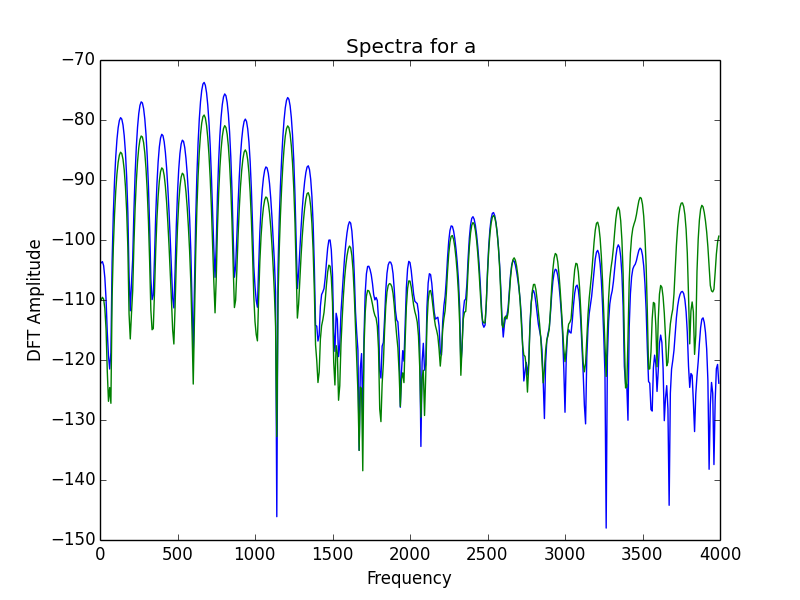
\includegraphics[width=\linewidth]{./images/spectra_a.png}
    \caption{ \textbackslash a\textbackslash from the natural recording of \textit{machali}}
    \label{fig:1}
\end{figure}


\begin{figure}[h!]
    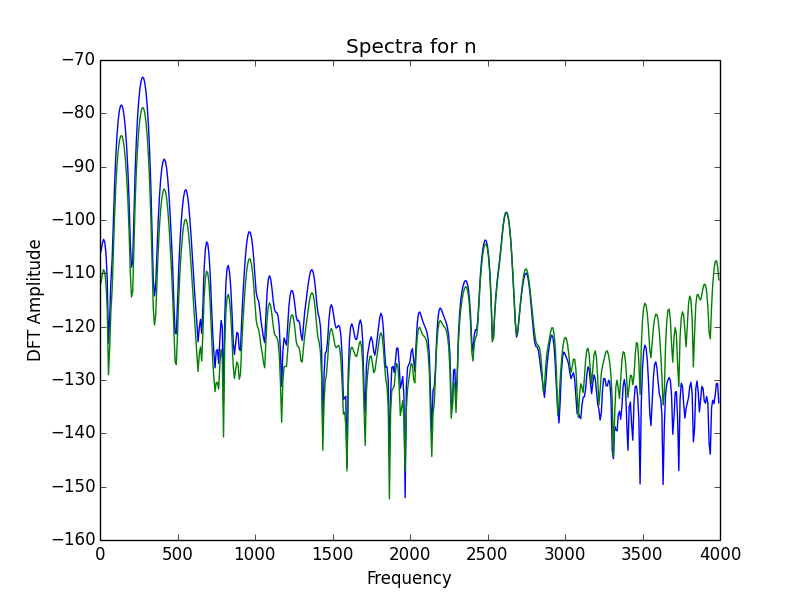
\includegraphics[width=\linewidth]{./images/spectra_n.png}
    \caption{ \textbackslash n\textbackslash from the natural recording of \textit{machali}}
    \label{fig:1}
\end{figure}




\begin{figure}[h!]
    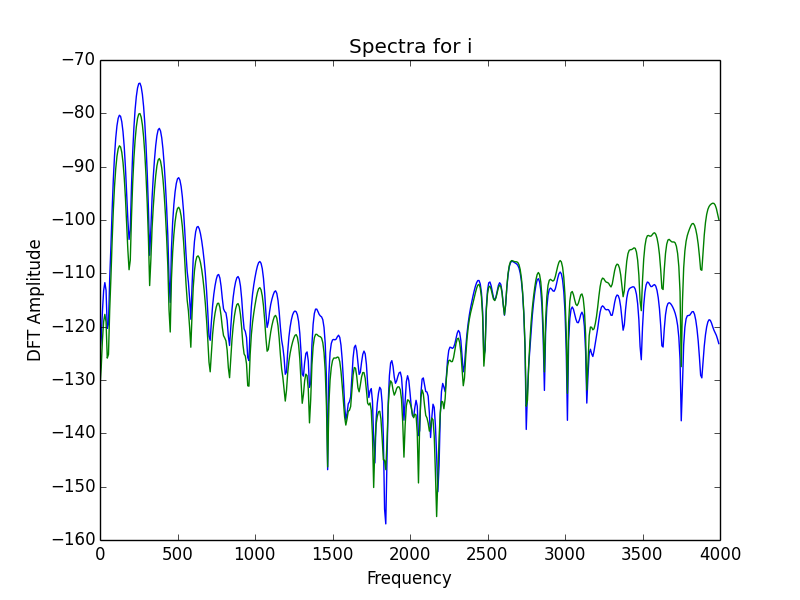
\includegraphics[width=\linewidth]{./images/spectra_i.png}
    \caption{\textbackslash I\textbackslash from the natural recording of \textit{machali}}
    \label{fig:1}
\end{figure}


\begin{figure}[h!]
    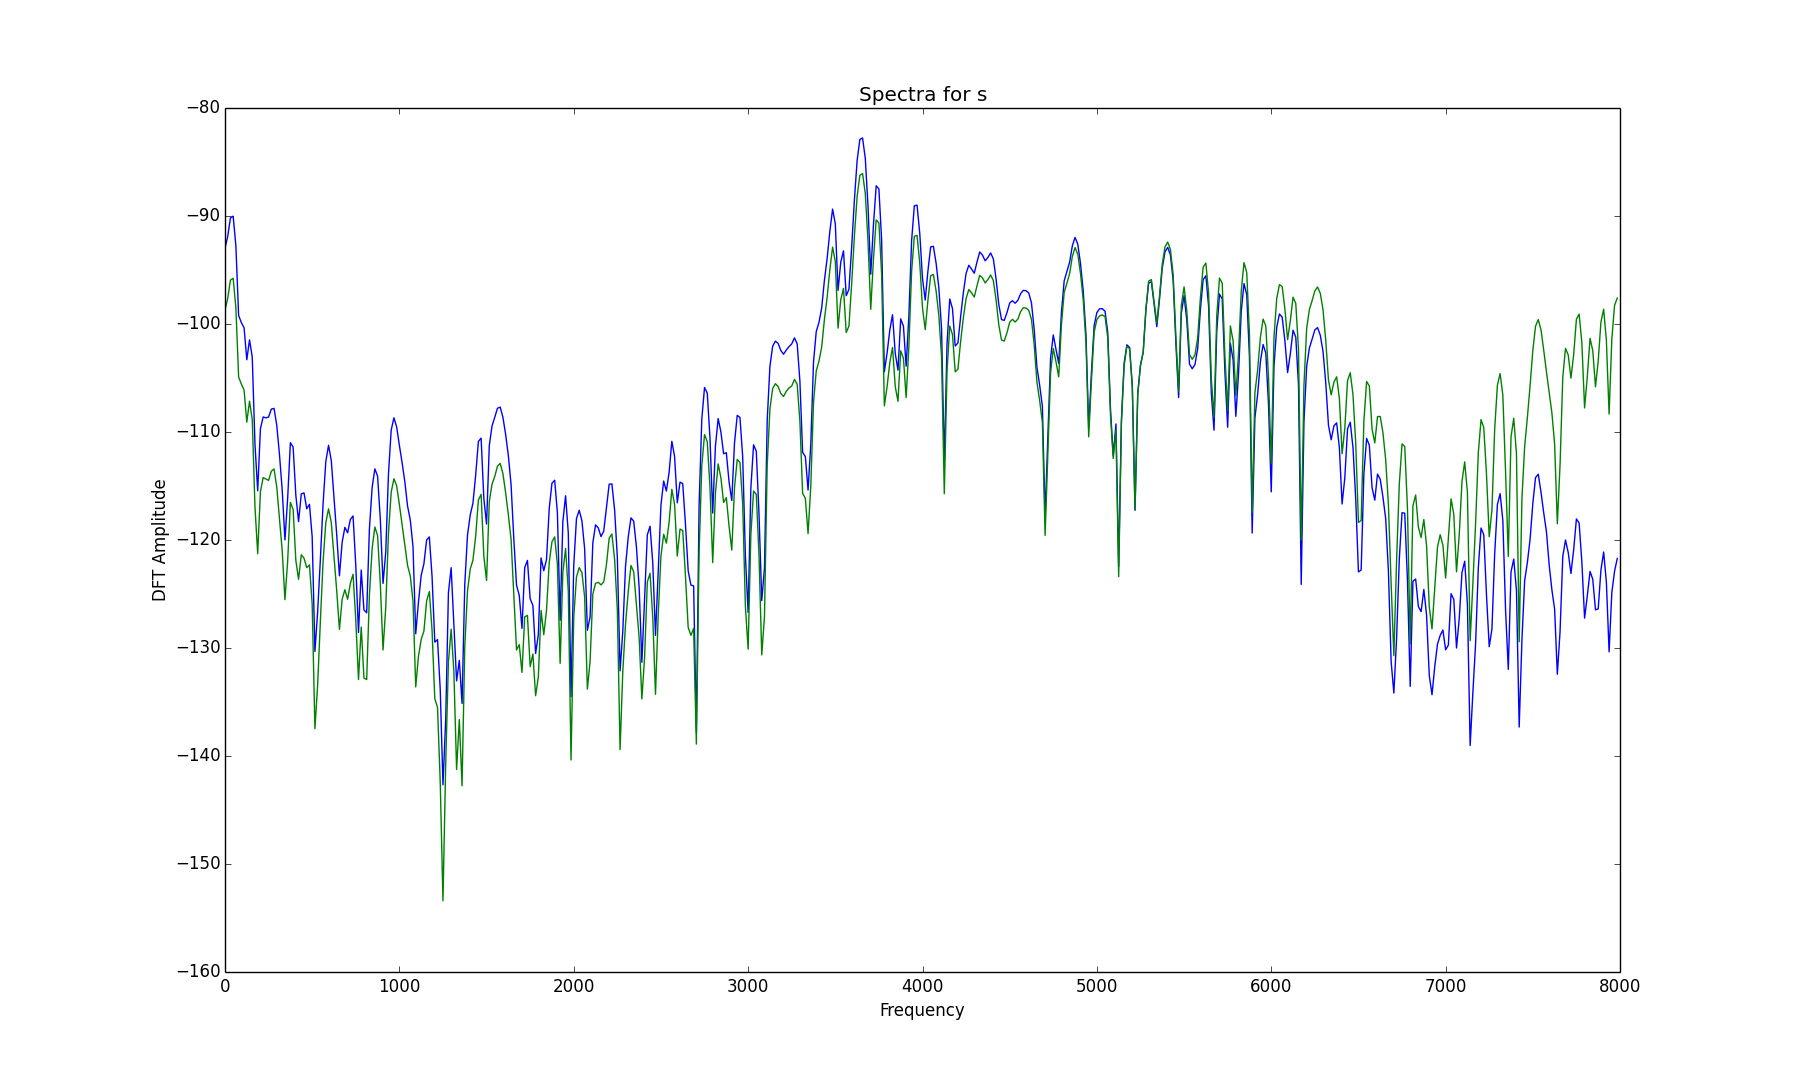
\includegraphics[width=\linewidth]{./images/spectra_s.png}
    \caption{ \textbackslash s\textbackslash from the natural recording of \textit{machali}}
    \label{fig:1}
\end{figure}



\newpage
\textbf{Poles and Zeros}

\begin{figure}[h!]
    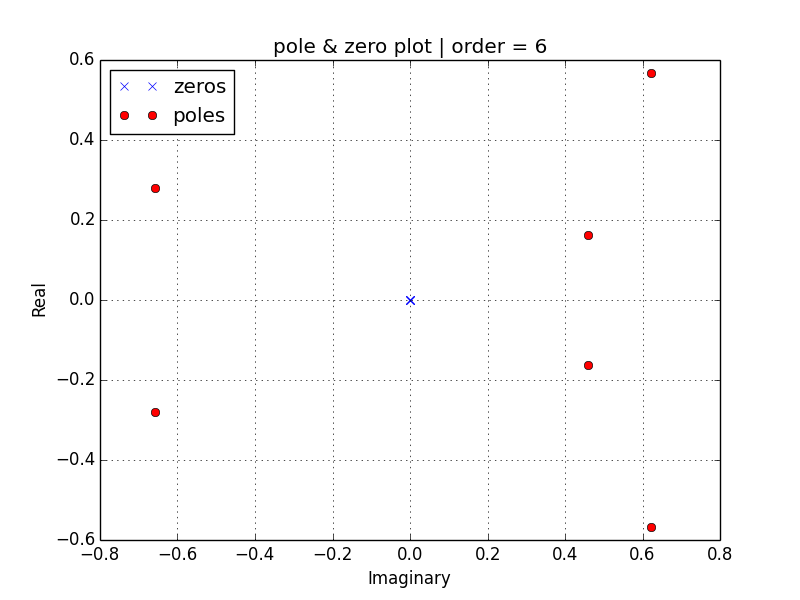
\includegraphics[width=\linewidth]{./images/a_pole-zero_6_.png}
    \caption{Poles and zeros when order = 6 for \textbackslash a\textbackslash from the natural recording of \textit{machali}}
    \label{fig:1}
\end{figure}


\begin{figure}[h!]
    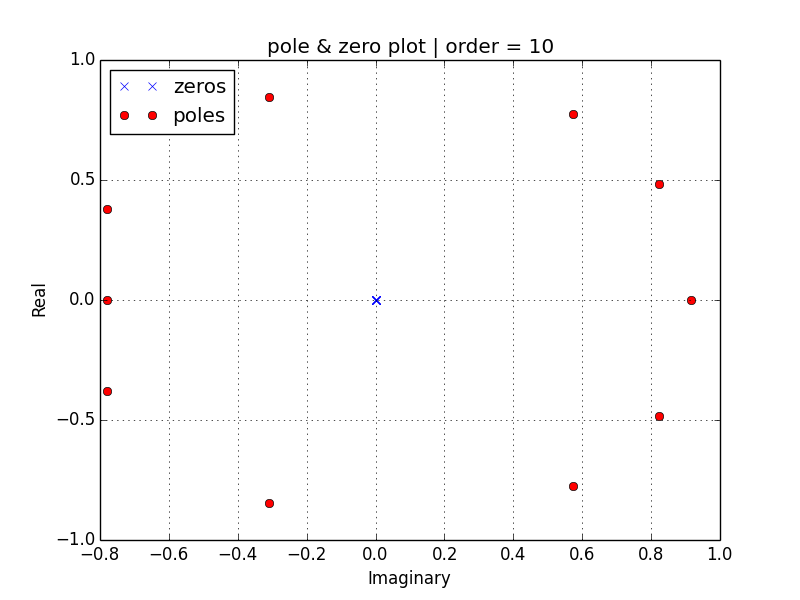
\includegraphics[width=\linewidth]{./images/a_pole-zero_10_.png}
    \caption{Poles and zeros when order = 10 for \textbackslash a\textbackslash from the natural recording of \textit{machali}}
    \label{fig:1}
\end{figure}




\begin{figure}[h!]
    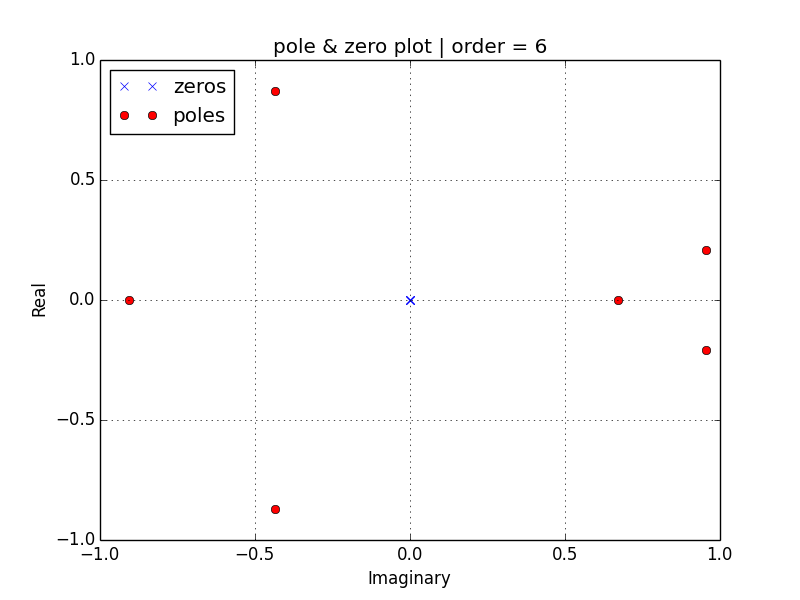
\includegraphics[width=\linewidth]{./images/n_pole-zero_6_.png}
    \caption{Poles and zeros when order = 6 for \textbackslash n\textbackslash from the natural recording of \textit{machali}}
    \label{fig:1}
\end{figure}


\begin{figure}[h!]
    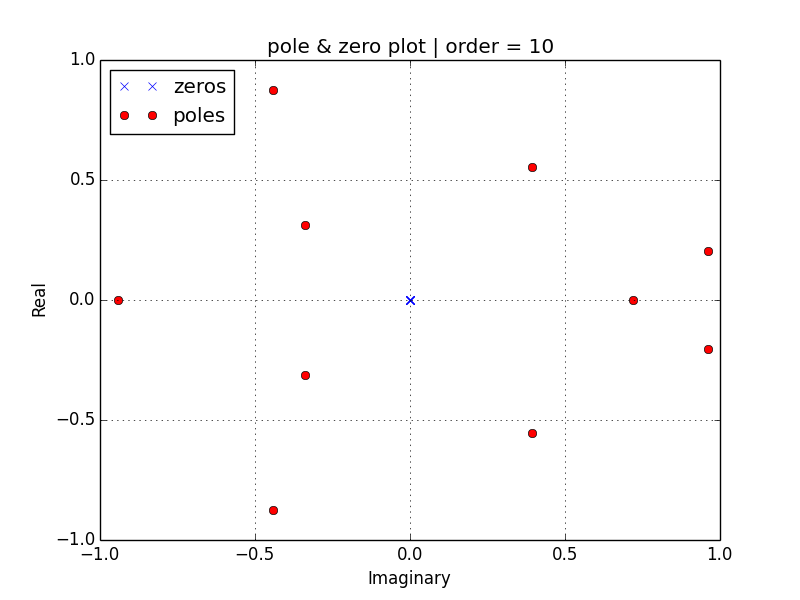
\includegraphics[width=\linewidth]{./images/n_pole-zero_10_.png}
    \caption{Poles and zeros when order = 10 for \textbackslash n\textbackslash from the natural recording of \textit{machali}}
    \label{fig:1}
\end{figure}




\begin{figure}[h!]
    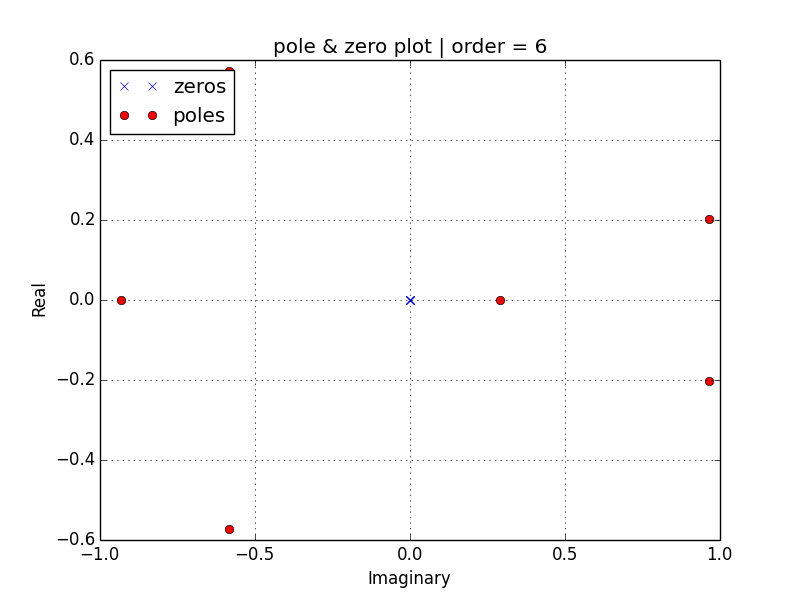
\includegraphics[width=\linewidth]{./images/i_pole-zero_6_.png}
    \caption{Poles and zeros when order = 6 for \textbackslash i\textbackslash from the natural recording of \textit{machali}}
    \label{fig:1}
\end{figure}


\begin{figure}[h!]
    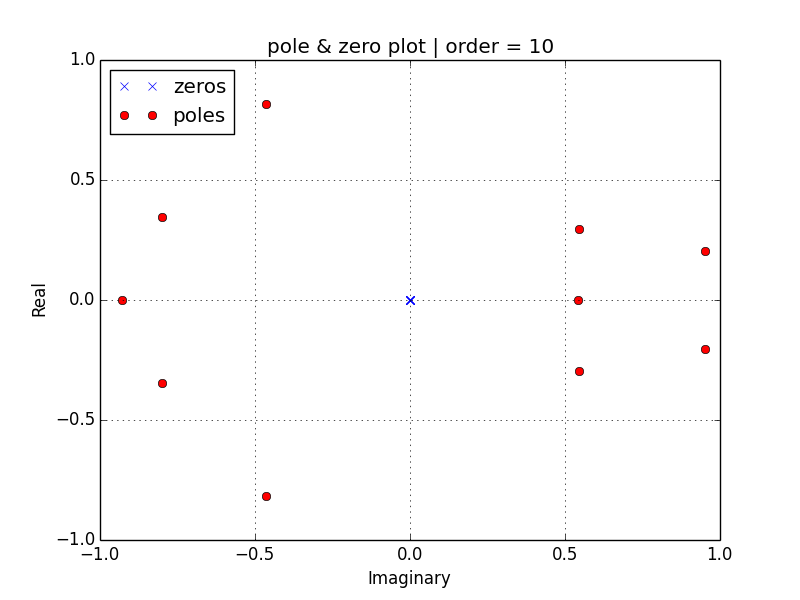
\includegraphics[width=\linewidth]{./images/i_pole-zero_10_.png}
    \caption{ Poles and zeros when order = 10 for \textbackslash i\textbackslash from the natural recording of \textit{machali}}
    \label{fig:1}
\end{figure}




\begin{figure}[h!]
    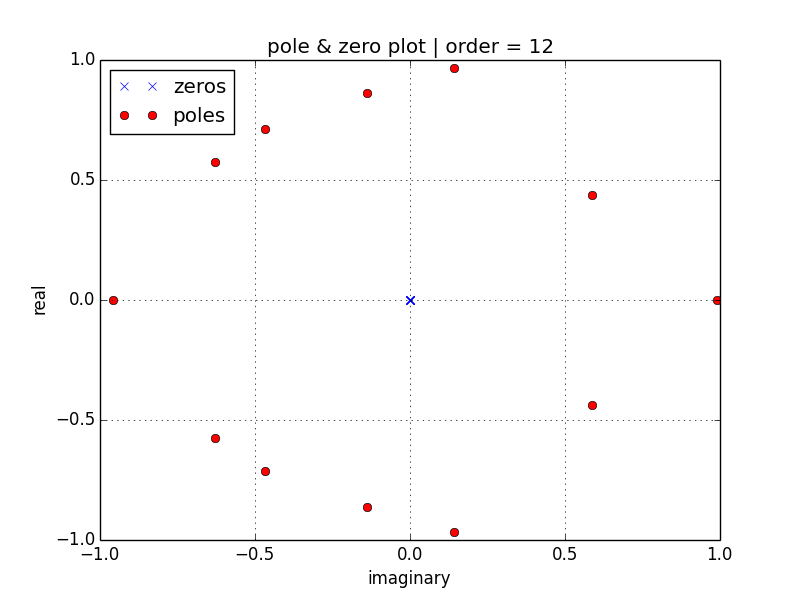
\includegraphics[width=\linewidth]{./images/s_pole-zero_12_.png}
    \caption{Poles and zeros when order = 12 for \textbackslash s\textbackslash from the natural recording of \textit{machali}}
    \label{fig:1}
\end{figure}


\begin{figure}[h!]
    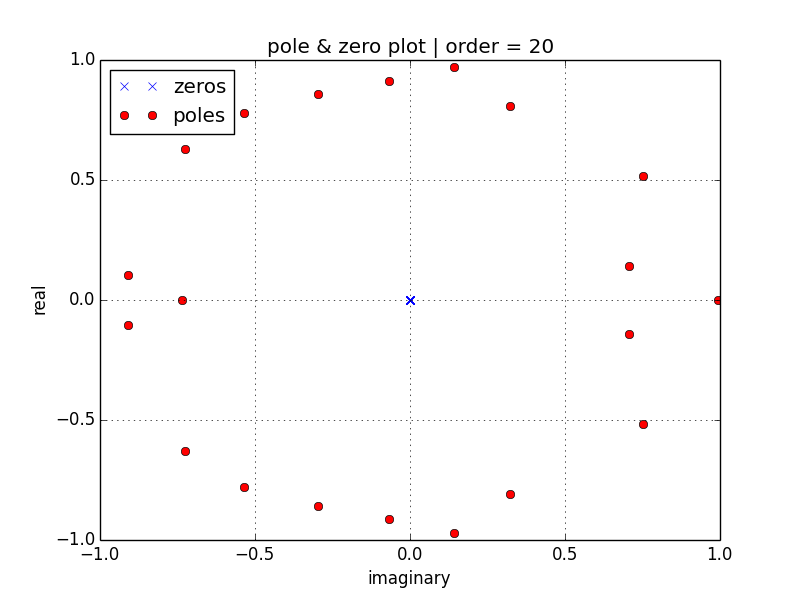
\includegraphics[width=\linewidth]{./images/s_pole-zero_20_.png}
    \caption{ Poles and zeros when order = 20 for \textbackslash s\textbackslash from the natural recording of \textit{machali}}
    \label{fig:1}
\end{figure}



\newpage

\textbf{Linear Predictive Coding Spectrum}


The gain for \textbackslash a\textbackslash from the natural recording of \textit{machali} is: 
\begin{itemize}
\item Order 2: 15.30 
\item Order 4: 13.13
\item Order 6: 12.84
\item Order 8: 12.42
\item Order 10: 10.99
\item Order 12: 10.47
\item Order 20: 10.07
\end{itemize}    

\begin{figure}[h!]
    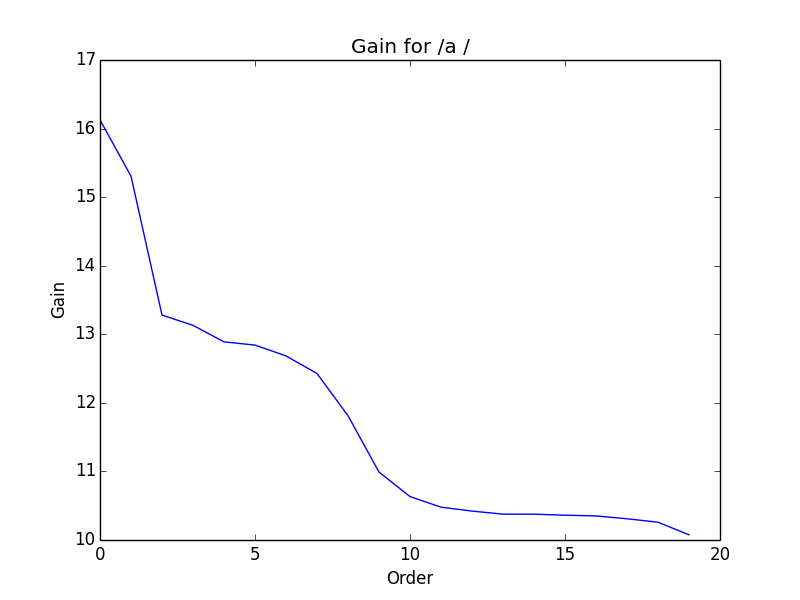
\includegraphics[width=\linewidth]{./images/gain_a.png}
    \caption{Gain of \textbackslash a\textbackslash from the natural recording of \textit{machali}}
    \label{fig:1}
\end{figure}

 
 

 
 

The gain for \textbackslash n\textbackslash from the natural recording of \textit{machali} is: 

\begin{itemize}
\item Order 2: 39.31 
\item Order 4: 24.83
\item Order 6: 17.51
\item Order 8: 17.07
\item Order 10: 17.00
\item Order 12: 16.58
\item Order 20: 16.12
\end{itemize}  
\begin{figure}[h!]
    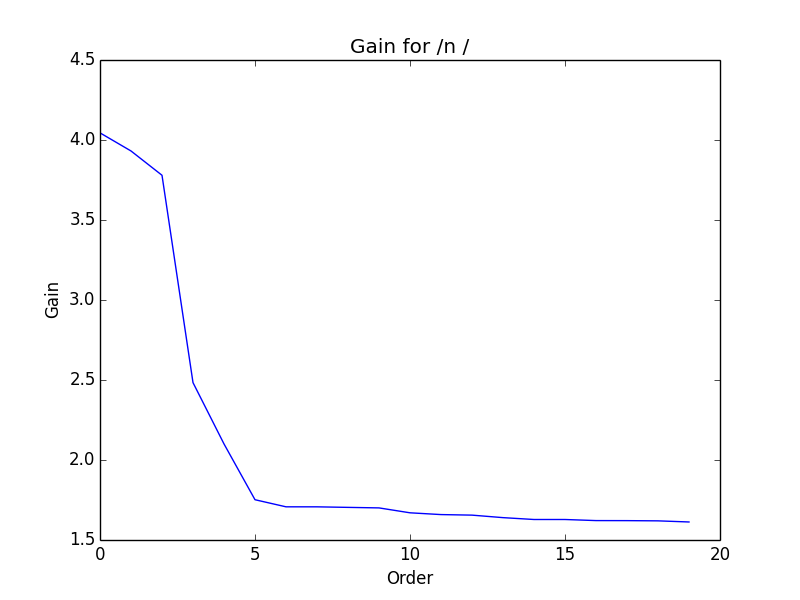
\includegraphics[width=\linewidth]{./images/gain_n.png}
    \caption{Gain of \textbackslash n\textbackslash from the natural recording of \textit{machali}}
    \label{fig:1}
\end{figure}


The gain for \textbackslash I\textbackslash from the natural recording of \textit{machali} is: 
\begin{itemize}
\item Order 2: 50.79 
\item Order 4: 28.53
\item Order 6: 25.04
\item Order 8: 22.36
\item Order 10: 21.19
\item Order 12: 21.05
\item Order 20: 19.42
\end{itemize}  


\begin{figure}[h!]
    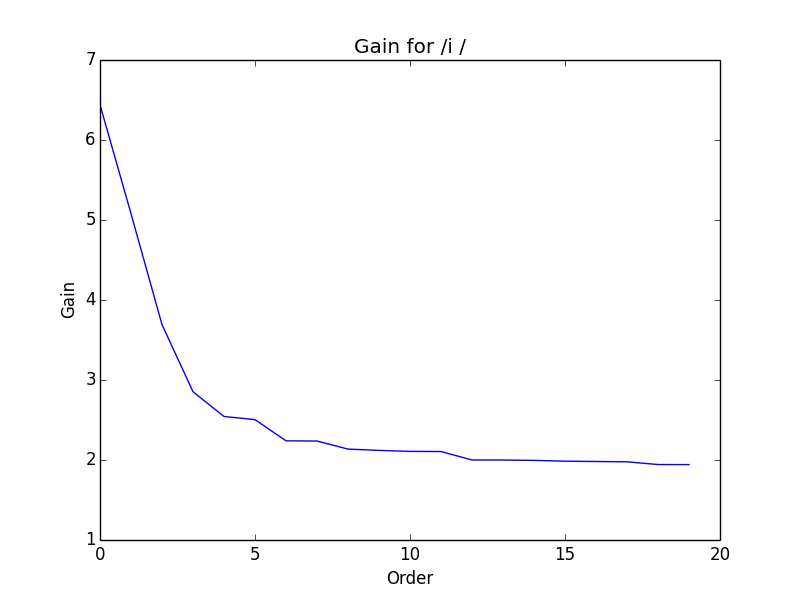
\includegraphics[width=\linewidth]{./images/gain_i.png}
    \caption{Gain of \textbackslash I\textbackslash from the natural recording of \textit{machali}}
    \label{fig:1}
\end{figure}

The gain for \textbackslash s\textbackslash from the natural recording of \textit{machali} is: 

\begin{itemize}
\item Order 2: 67.89 
\item Order 4: 65.96
\item Order 6: 45.62
\item Order 8: 39.59
\item Order 10: 39.07
\item Order 12: 38.32
\item Order 20: 36.29
\end{itemize}  


\begin{figure}[h!]
    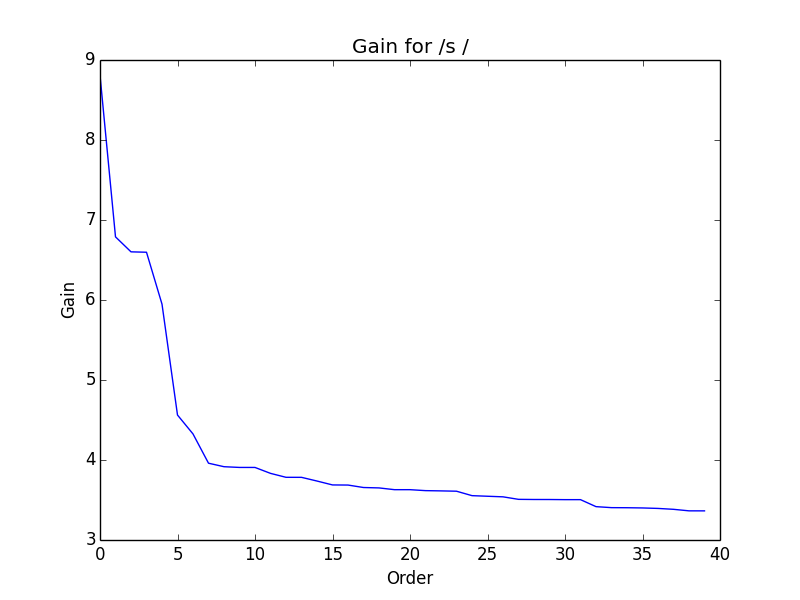
\includegraphics[width=\linewidth]{./images/gain_s.png}
    \caption{Gain of \textbackslash s\textbackslash from the natural recording of \textit{machali}}
    \label{fig:1}
\end{figure}



\newpage

\textbf{Error signal energy}

\begin{figure}[h!]
    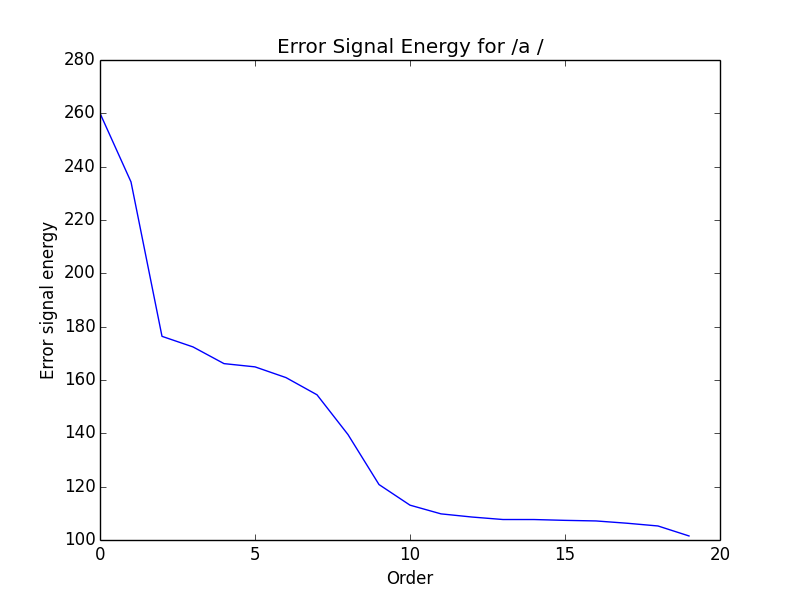
\includegraphics[width=\linewidth]{./images/error_energy_a.png}
    \caption{Error Signal Energy for \textbackslash i\textbackslash from the natural recording of \textit{machali}}
    \label{fig:1}
\end{figure}


\begin{figure}[h!]
    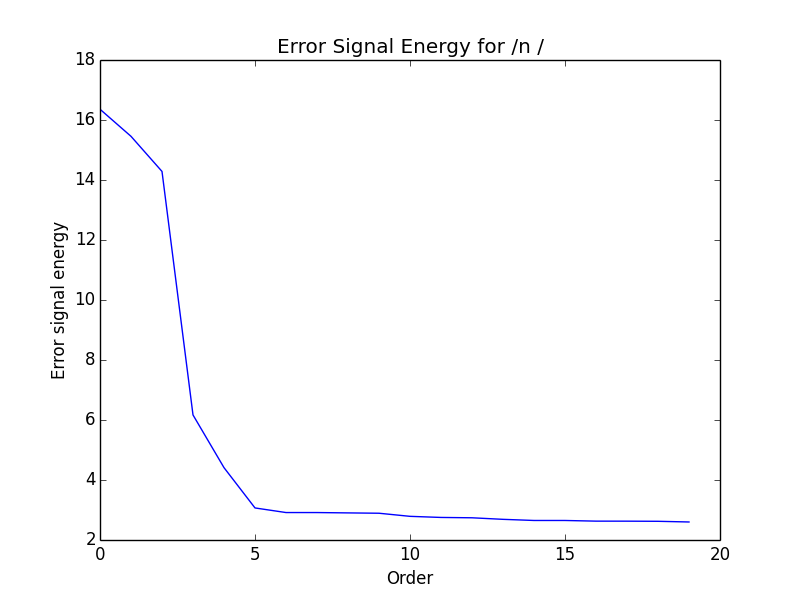
\includegraphics[width=\linewidth]{./images/error_energy_n.png}
    \caption{Error Signal Energy for \textbackslash i\textbackslash from the natural recording of \textit{machali}}
    \label{fig:1}
\end{figure}




\begin{figure}[h!]
    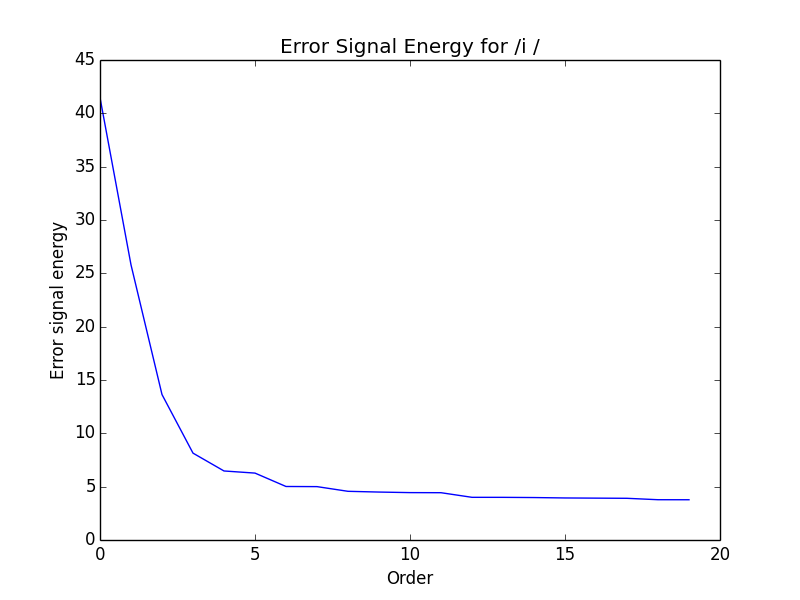
\includegraphics[width=\linewidth]{./images/error_energy_i.png}
    \caption{Error Signal Energy for \textbackslash s\textbackslash from the natural recording of \textit{machali}}
    \label{fig:1}
\end{figure}


\begin{figure}[h!]
    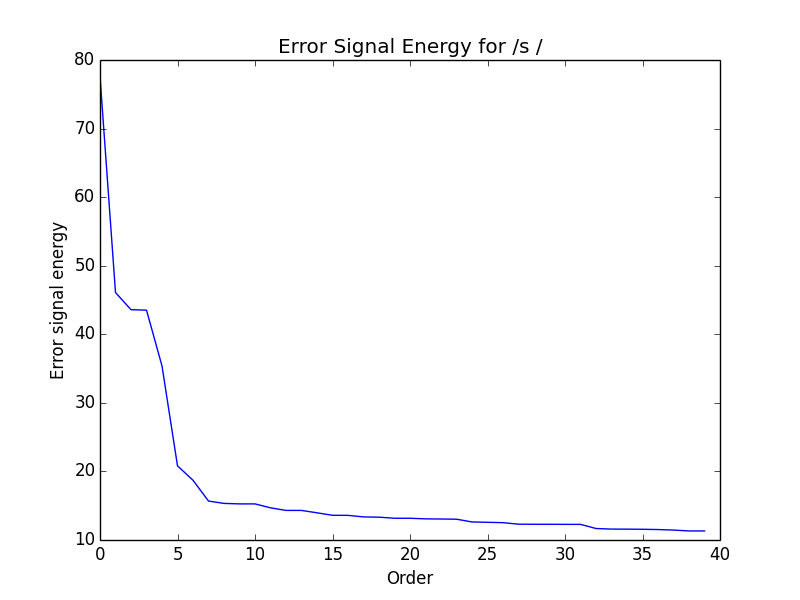
\includegraphics[width=\linewidth]{./images/error_energy_s.png}
    \caption{ Error Signal Energy for \textbackslash s\textbackslash from the natural recording of \textit{machali}}
    \label{fig:1}
\end{figure}


\newpage
\section{Question 3}
Based on the $10$th-order LPCs, carry out the inverse filtering of the  \textbackslash a\textbackslash vowel segment and of the unvoiced sound  \textbackslash s\textbackslash. Obtain the residual error signal in each case. Can you measure the pitch period of the voiced sound from the residual waveform? Use the acf to detect the pitch. Plot the magnitude spectrum of each of the residual signals. 

\subsection{Answer}


\textbf{}

\begin{figure}[h!]
    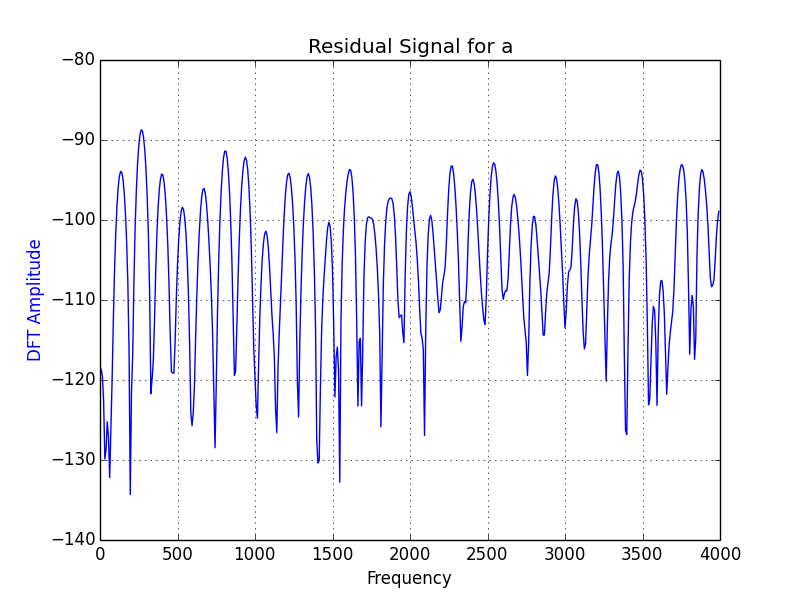
\includegraphics[width=\linewidth]{./images/res_signal_a.png}
    \caption{Residual signal  for \textbackslash a\textbackslash from the natural recording of \textit{machali}}
    \label{fig:1}
\end{figure}


\begin{figure}[h!]
    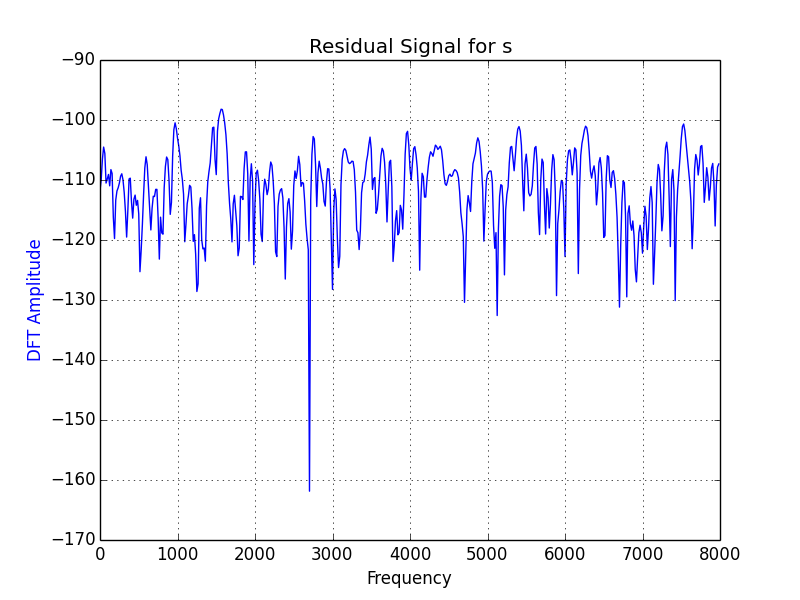
\includegraphics[width=\linewidth]{./images/res_sig_s.png}
    \caption{Residual signal for \textbackslash s\textbackslash from the natural recording of \textit{machali}}
    \label{fig:1}
\end{figure}




\begin{figure}[h!]
    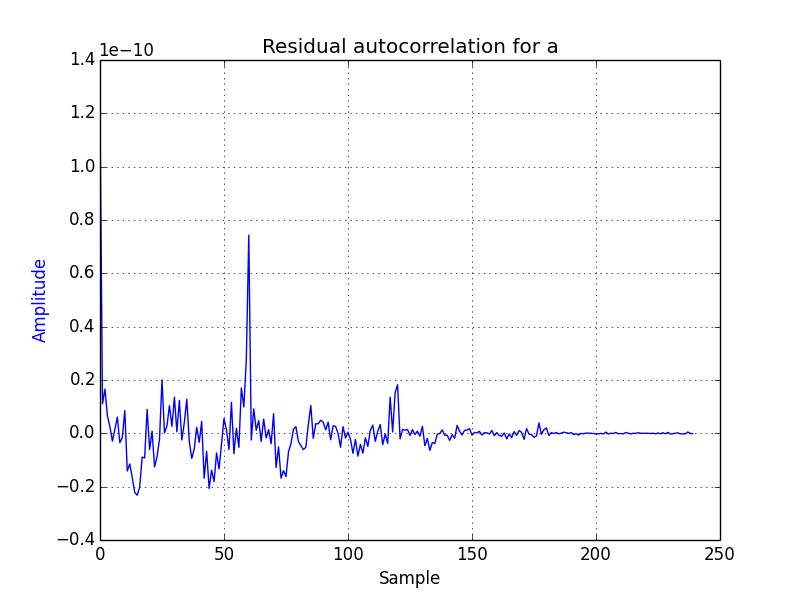
\includegraphics[width=\linewidth]{./images/res_autocorr_a.png}
    \caption{Autocorrelation of the residual signal for  \textbackslash a\textbackslash from the natural recording of \textit{machali}}
    \label{fig:1}
\end{figure}


\begin{figure}[h!]
    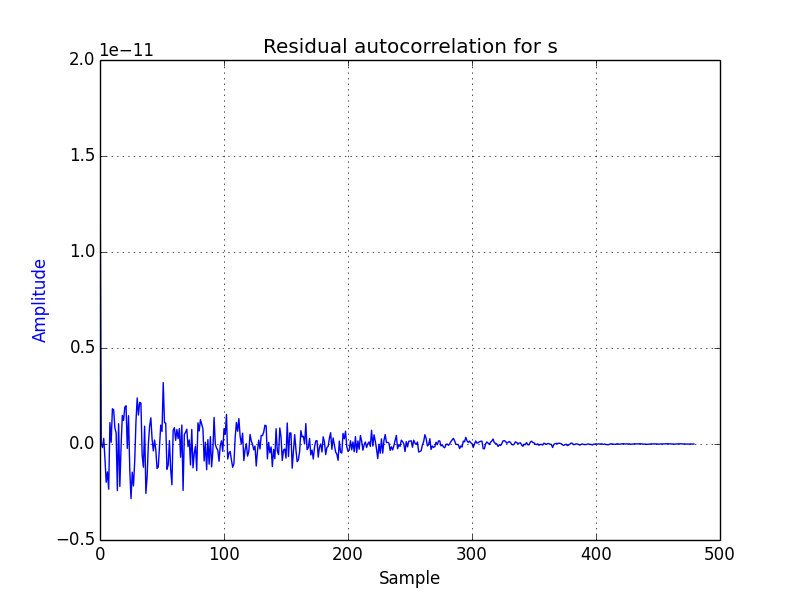
\includegraphics[width=\linewidth]{./images/res_autocorr_s.png}
    \caption{Autocorrelation of the residual signal for \textbackslash s\textbackslash from the natural recording of \textit{machali}}
    \label{fig:1}
\end{figure}

From the figure, we can see that the autocorrelation function for \textbackslash a\textbackslash achieves a maxima (spike) at around 60 samples. Given that the sampling rate is $8$ KHz, the pitch of the signal should be $8000/60 = 133.33$ Hz. \\
We could do this since \textbackslash a\textbackslash is a voicde sound. On the other hand, \textbackslash s\textbackslash is an unvoiced sound and hence we can't observe any maxima in it't autocorrelation function. Hence we cannot calculate a pitch for this sound. 

\textbf{Spectrum of residual signals}

\begin{figure}[h!]
    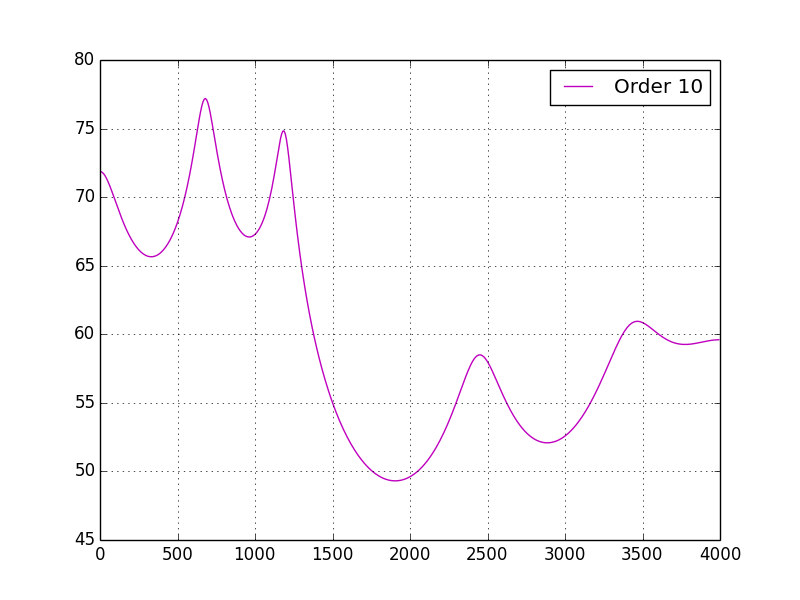
\includegraphics[width=\linewidth]{./images/res_spec_a.png}
    \caption{Spectrum of the residual signal for  \textbackslash a\textbackslash from the natural recording of \textit{machali}}
    \label{fig:1}
\end{figure}


\begin{figure}[h!]
    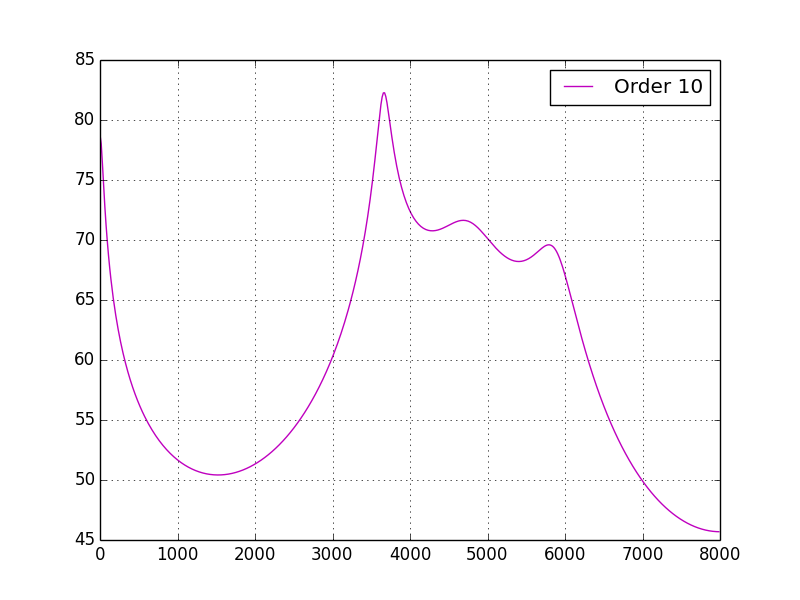
\includegraphics[width=\linewidth]{./images/res_spec_s.png}
    \caption{Spectrum of the residual signal for \textbackslash s\textbackslash from the natural recording of \textit{machali}}
    \label{fig:1}
\end{figure}


\end{document}